\chapter{Implementation and simulation}

The release comes with an initial Vivado 2019.2 project under Windows. When opening the \$project/vivado/fpga\_top/fpga\_top.xpr project, it can be seen, that the project is not compiled yet. The project can be compiled by clicking on the ''Generate Bitstream'' link. It will roughly take 30 minutes or so. Alternatively, the precompiled ''bit'' file \$project/bit/fpga\_top.bit can be used for downloading.

The project has been developed using version 2017.2. After testing the release using various versions (2018.2, 2019.2) it turned out, that there are too many variations. 2018.2 gives me an overmapped (103\% LUT) error for unknown reasons and 2019.2 didn't make the timing at that time. So the project is released using the latest version 2019.2 and the timing is clean now.

The design hierarchy can be seen in Fig. \ref{hierarchy}. The parameters are stored in MPSOC\_parameter. The rest is pretty much self-explaining. The ''\_syn'' memory files are used for synthesis. The memory files also have a bypass data register implemented to improve the RAMs write-through capabilities.

The ''clk\_100M'' module converts the incoming 100 MHz clock into an internal 180 MHz clock.

\begin{figure*}[!t]
	\centering
	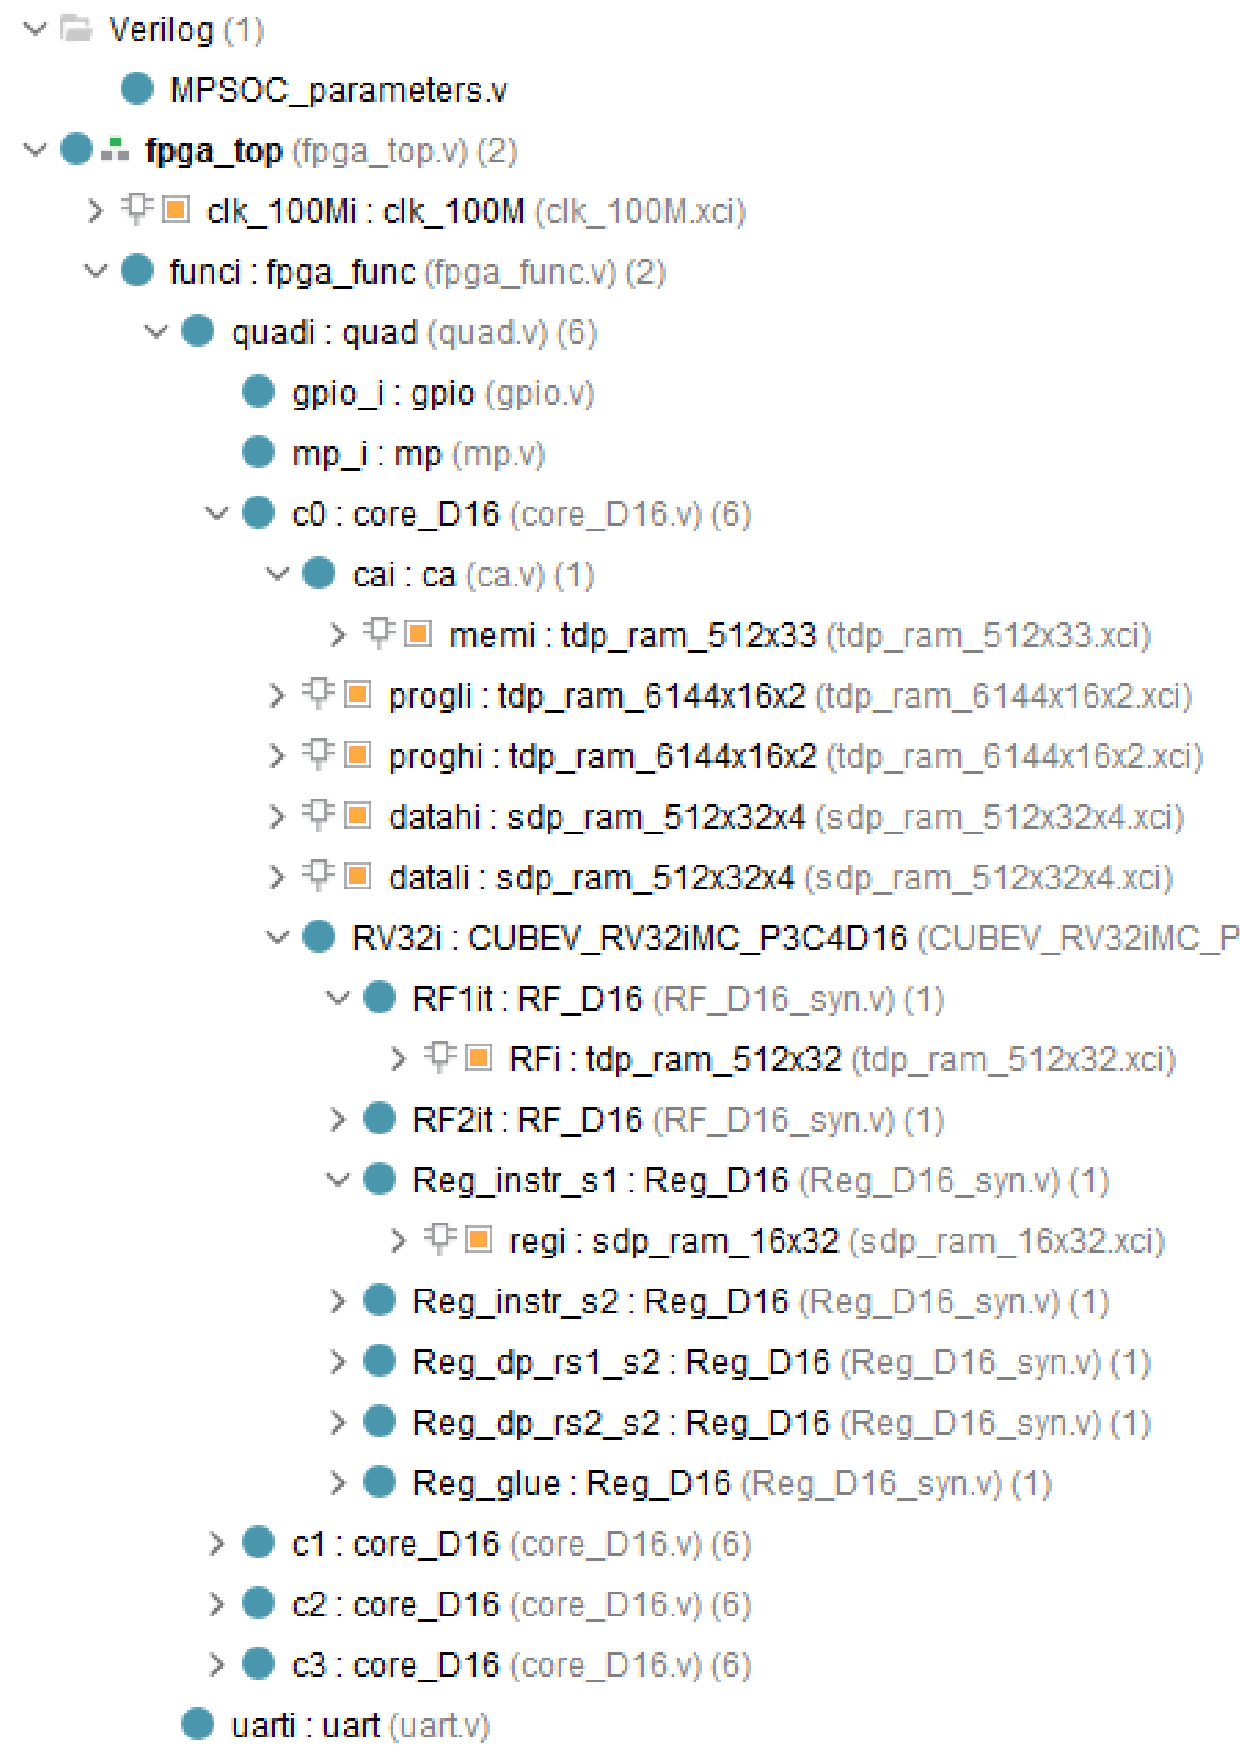
\includegraphics[width=6in]{figs/hierarchy}
	\caption{Overview of the design hierarchy.}
	\label{hierarchy}
\end{figure*}


This Vivado project also has a top level simulation setup ''tb\_top''. It simulates the complete FPGA but without the clk\_100M module. It tests the UART connectivity, data and program memory write and read as well as reset functionality. It also downloads a program which writes and reads some UART data.

There are two additional Vivado simulation projects. One project ''\$project/vivado/simulation\_CUBEV'' simulates the CUBE-V core, by executing all instructions and by running some CHStone tests, the other project ''\$project/vivado/simulation\_quad'' tests 4 CUBE-V instantiations at the same time, their individual system features and how they interact with each other or with the GPIO peripheral. 

All simulation so far are self-testing. There are additional demo-tests in the ''simulation\_quad'' project, which  demonstrate the usage of multithreaded drivers.
